%-------------------------------------------------------------------------------
% Autores: I. R. Pagnossin e Centro de Ensino e Pesquisa Aplicada.
%
% Este material é parte integrante do curso "Usando LaTeX; pensando em TeX" e é
% distribuido pelos autores segundo a licença Creative Commons 2.5 Brasil
% (atribuição/não-comercial/redistribuição segundo a mesma licença).
%
% This material is part of the course "Usando LaTeX; pensando em TeX".
% It is distributed according to the license Creative Commons 2.5 Brazil
% (atribution/non-comercial use/share alike the same license).
%-------------------------------------------------------------------------------
\newif\ifhandout
%\handouttrue  % Descomente se for para gerar a versão para IMPRESSÃO.
\handoutfalse % Descomente se for para gerar a versão para APRESENTAÇÃO

%-------------------------------------------------------------------------------
\ifhandout
  \documentclass[handout,10pt]{beamer}
  \mode<handout>
\else
	\documentclass[10pt,hyperref={pdfpagelabels=false}]{beamer}
	\mode<presentation>
\fi

	\usepackage[utf8]{inputenc}
	\usepackage{ae}	
	\usepackage[brazil]{babel}	
	\usepackage{graphicx}
	\usepackage{listings}
	\usepackage{tikz}
	\usepackage{amsmath}
	\usepackage[squaren]{SIunits}
	\usepackage{booktabs}
	\usepackage{fancybox}
	\usepackage{array}
	
	\ifhandout
		\usepackage{pgfpages}
		\pgfpagesuselayout{2 on 1}[a4paper,border shrink=5mm]
	\fi
	
	

	\usetikzlibrary{shapes.symbols}


	% Configurações pessoais
	% Configurações personalizadas do código LaTeX.	
\lstnewenvironment{LaTeXcode}{
	\setlength{\abovecaptionskip}{0pt}	
	\lstset{language=[LaTeX]TeX}
	\lstset{%
		basicstyle=\footnotesize\ttfamily,  % Global
		keywordstyle=\color{blue}\bfseries, % Comandos
		identifierstyle=,                   % Texto
		stringstyle=,                       % Strings 
		commentstyle=\color{gray},          % Comentários
		showstringspaces=false,             % Espaços
		rulecolor=\color{gray},             % Linha da caixa
	}
	\lstset{emph={setlength,includegraphics,psfrag,subfigure},emphstyle={\color{blue}\bfseries}}
}% Abrindo o ambiente.
{}% Fechando o ambiente.
	
\newcommand{\digite}[1]{{\fontfamily{cmss}\fontseries{bx}\selectfont#1}}	
\newcommand{\cs}[1]{{\normalfont\textbackslash\color{blue!50!black}#1}}
\newcommand{\pkg}[1]{{\normalfont\sffamily\color{orange}#1}}
\newcommand{\env}[1]{{\normalfont\sffamily\color{green!50!black}#1}}
\let\comando=\cs
\let\package=\pkg
\let\ambiente=\env
\newcommand{\foreign}[1]{{\textsl{#1}}}


	\newcounter{exercicio}	
	\newenvironment{exercicio}{%
		\refstepcounter{exercicio}%
		\penalty-200
		\noindent\colorbox{blue!60!black}{\makebox[\columnwidth-\fboxsep*2][c]{\textbf{\color{white}Exercício~\theexercicio}}}\smallskip
	}{\par\medskip}
		

\newcommand{\bibtex}{\textsc{Bib}\TeX}

\newenvironment<>{atividade}[1]{%
\begin{actionenv}#2%
\begin{exampleblock}{{Atividade #1}}%
}
{%
\end{exampleblock}%
\end{actionenv}%
}


	% Path das figuras, relativo a esta pasta.
	\graphicspath{{../arquivos_comuns/figuras/}{./figuras/}}

	% Modelo da apresentação	
	\usetheme{Frankfurt}
	\usefonttheme{serif,structurebold}
	\setbeamercovered{transparent}
	
	% Comandos personalizados especialmente para esta apresentação.
	\newcommand{\frfamily}{\fontfamily{cmfr}\selectfont}
	\newcommand{\tmfamily}{\fontfamily{ptm}\selectfont}
	\newcommand{\plfamily}{\fontfamily{ppl}\selectfont}
	\newcommand{\hvfamily}{\fontfamily{phv}\selectfont}
	\newcommand{\agfamily}{\fontfamily{pag}\selectfont}
	\newcommand{\zcfamily}{\fontfamily{pzc}\selectfont}
	\newcommand{\familycode}[1]{{\ttfamily#1}}
	\newcommand{\mhelvetica}[1]{{\fontfamily{phv}\fontseries{m}\selectfont#1}}
	\newcommand{\bhelvetica}[1]{{\fontfamily{phv}\fontseries{b}\selectfont#1}}
	\newcommand{\bxhelvetica}[1]{{\fontfamily{phv}\fontseries{bx}\selectfont#1}}
	\newcommand{\mchelvetica}[1]{{\fontfamily{phv}\fontseries{mc}\selectfont#1}}
	\newcommand{\bchelvetica}[1]{{\fontfamily{phv}\fontseries{bc}\selectfont#1}}	
	
	% Metadados do arquivo PDF.
	\hypersetup{
		pdftitle={Fontes I - as famílias Computer Modern},
		pdfauthor={Dr. Ivan R. Pagnossin},
		pdfsubject={LaTeX},
		pdfkeywords={TeX,LaTeX}
	}

	% Título, autores e instituição.
	\title{Fontes I}
	\subtitle{As famílias Computer Modern}
	
	\author{\textbf{Prof.:} Ivan R. Pagnossin \and \textbf{Tutora:} Juliana Giordano}
	\institute{%
		Coordenadoria de Tecnologia da Informação\\
		Centro de Ensino e Pesquisa Aplicada}
	\logo{
\includegraphics[width=0.25\textwidth]{LogotipoCursoLaTeX_v3_pequeno}}
	\date{}
	
\begin{document}


%-------------------------------------------------------------------
\begin{frame}[c,label=titulo]
	\centering	
	
	
\includegraphics[width=0.8\textwidth]{LogotipoCursoLaTeX_v2}

	\titlepage
\end{frame}

\logo{} % <-- O logotipo não aparecerá mais a partir daqui.
\setbeamertemplate{background canvas}{%
		
\includegraphics[width=\paperwidth,height=\paperheight,keepaspectratio=false]{leao-pensador-wattermark.png}
}

%-------------------------------------------------------------------
\section{Pacotes}
\begin{frame}[fragile,c]
	\frametitle{Pacotes}
	\framesubtitle{O pacote \pkg{inputenc}}

	\centering

	Pacotes são recursos extras que podem ser utilizados pelo compilador (\LaTeX).
	Eles são carregados na memória com este comando:
	
	\vfill
	
	\begin{block}{}
		No \textbf{preâmbulo} escreva:
		\cs{usepackage}[\textit{opções}]\{\textit{nome do pacote}\}
	\end{block}\vfill
	
	\begin{atividade}<2->{1}
		%
		\begin{LaTeXcode}		  
			\documentclass{article}
			  \usepackage[utf8]{inputenc}
			\begin{document}
			  Agora é possível acentuar o texto normalmente,
			  mas você ainda pode usar a acentua\c c\~ao
			  padr\~ao do \TeX, se quiser!
			\end{document}
		\end{LaTeXcode}		
	\end{atividade}\vfill


	\uncover<3->{\begin{center}
		\textbf{Atenção:} \cs{usepackage} só pode ser utilizado no \emph{preâmbulo}.
	\end{center}}

\end{frame}
%-------------------------------------------------------------------
\section{Fontes}
\subsection{Codificações de entrada e de saída}
\begin{frame}
	\frametitle{Codificações de entrada e de saída}
	
	\vfill
	
	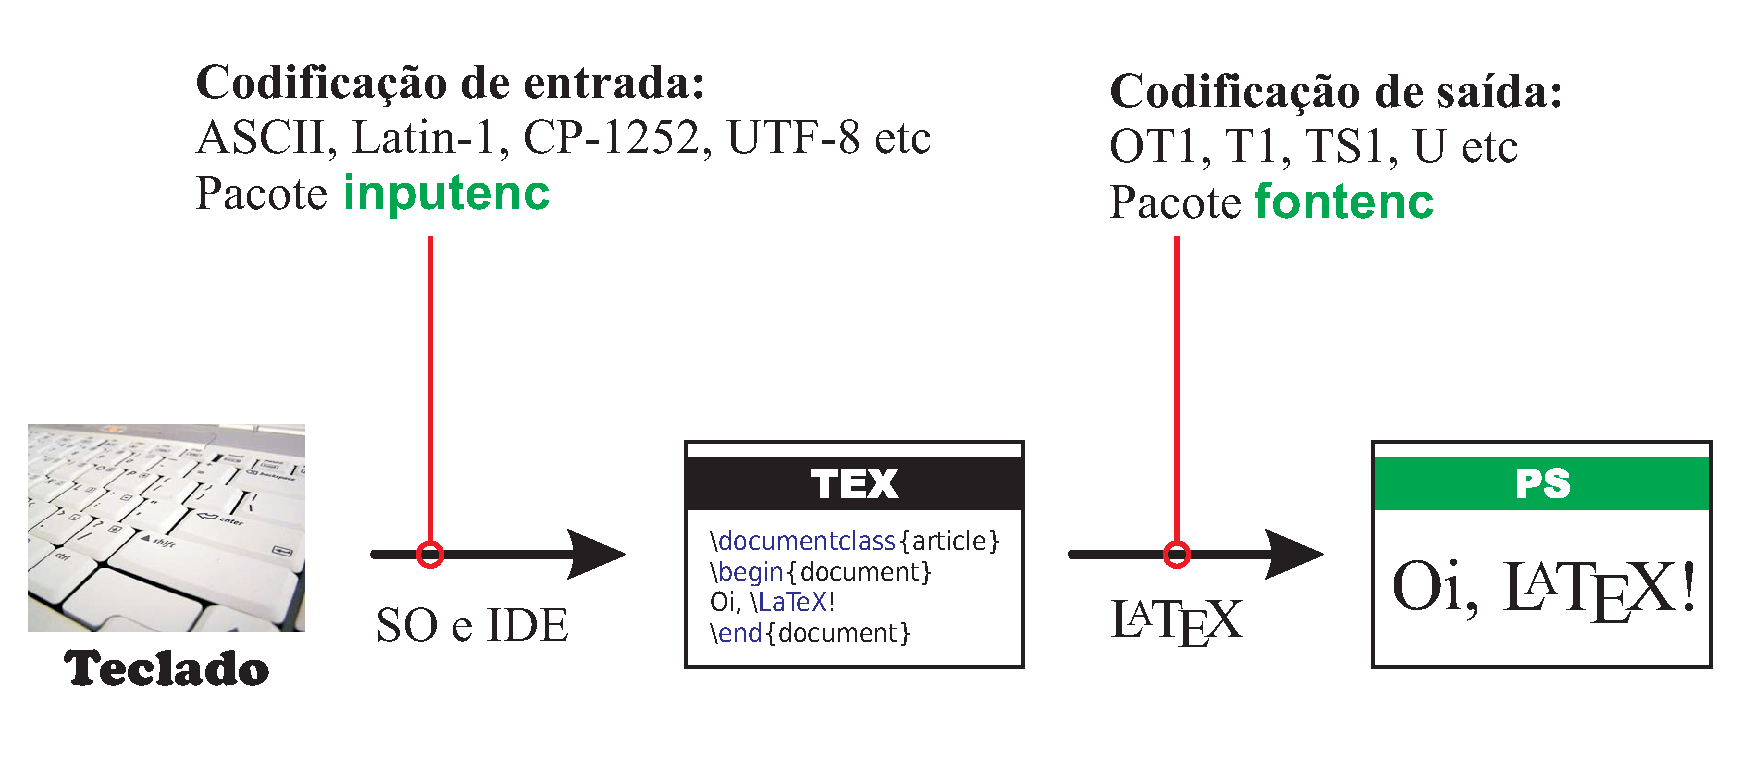
\includegraphics[width=\textwidth]{encodings}
	
	\vfill
	
	\footnotesize
	SO: Sistema operacional\\
	IDE: \foreign{Integrated Development Environment} (o TeXnicCenter)
	
\end{frame}
%-------------------------------------------------------------------
\subsection{Classificação no \LaTeX}
\begin{frame}
	\frametitle{Classificação de fontes}
		
	\begin{block}<1->{1. Codificação \alert{de saída} (\foreign{encoding})}
		\texttt{OT1}, \texttt{T1}, \texttt{TS1}, \texttt{OMS}, etc
	\end{block}\vfill

	\begin{block}<2->{2. Família (\foreign{family})}
		{\tmfamily Times}, {\zcfamily Zapf Chancery},
		{\hvfamily Helvetica}, {\frfamily Funny Roman}, {\agfamily Avant Garde}, etc
	\end{block}\vfill
	
	\begin{block}<3->{3. Série (\foreign{series}) \hfill $=\text{peso} + \text{largura}$}
		\mhelvetica{média}, \mchelvetica{média compacta}, \bhelvetica{negrito}, \bxhelvetica{negrito estendido}, etc
	\end{block}\vfill
	
	\begin{block}<4->{4. Forma (\foreign{shape})}
		\textup{normal}, \textsl{inclinado}, \textit{itálico}, ``\textsc{maiusculazinhas}''
	\end{block}\vfill	
	
	\begin{block}<5->{5. Tamanho (\foreign{size})}
		{\footnotesize pequeno}, médio, {\Large grande} etc.
	\end{block}
		
\end{frame}
%-------------------------------------------------------------------
\begin{frame}
	\frametitle{Classificação de fontes}
	\framesubtitle{Representação e exemplos}
	
	\begin{block}<1->{Classificação}
	\textsl{Codificação}/\textsl{Família}/\textsl{Série}/\textsl{Forma}/\textsl{Tamanho}	
	\end{block}
	
	\medskip
		
	\onslide<2->Exemplo de classificação:\\OT1/Computer Modern Roman/negrito estendido/itálico/\unit{5}{pt}
	
	\medskip
	
	\begin{block}<3->{Exercício 1}	
		\begin{itemize}
		\item<3,8-> T1/C.~M.~Sans-serif/médio/inclinado/\unit{10}{pt}\hfill{\usefont{T1}{cmss}{m}{sl}Exemplo}
		\item<4,8-> OT1/C.~M.~Funny Roman/médio/itálico/\unit{8.56}{pt}\hfill{\usefont{OT1}{cmfr}{m}{it}Exemplo}		
		\item<5,8-> T1/Times/negrito/maiusculazinhas/\unit{21}{pt}\hfill{\usefont{T1}{ptm}{b}{sc}Exemplo}
		\item<6,8-> T1/Avant Garde/negrito estendido/inclinado/\unit{10}{pt}\hfill{\usefont{T1}{pag}{bx}{sl}Exemplo}
		\item<7,8-> OT1/Bookman/negrito/normal/\unit{12}{pt}\hfill{\usefont{OT1}{pbk}{b}{n}Exemplo}
		\end{itemize}
		
		\medskip
		
		\footnotesize\textbf{obs.:} $\text{C.~M.} = \text{\foreign{Computer Modern}}$
	\end{block}
	
\end{frame}
%-------------------------------------------------------------------
\subsection{As famílias Computer Modern}
\begin{frame}
	\frametitle{Computer Modern (CM)}
	\framesubtitle{As fontes de D.~E.~Knuth}	
	
	\begin{enumerate}
	\item<1-> Codificação \alert{de saída}: OT1 (7 bits: 128 símbolos)
	
	\item<2-> Famílias:
		\begin{itemize}
		\item<2->\textrm{Computer Modern \alert<2->{R}o\alert<2->{m}an}\hfill \texttt{\alert{rm}}
		\item<3->\textsf{Computer Modern \alert<3->{S}ans Seri\alert<3->{f}}\hfill \texttt{\alert{sf}}
		\item<4->\texttt{Computer Modern \alert<4->{T}ypewri\alert<4->{t}er}\hfill \texttt{\alert{tt}}
		\end{itemize}
	
	\item<5-> Séries:
		\begin{itemize}
		\item<5->\textmd{Média} (\alert<5->{m}e\alert<5->{d}ium)\hfill \texttt{\alert{md}}
		\item<6->\textbf{Negrito expandido} (\alert<6->{b}old\alert<6->{f}ace)\hfill \texttt{\alert{bf}}
		\end{itemize}
	
	\item<7-> Forma:
		\begin{itemize}
		\item<7->\textup{Normal (\alert<7->{up}right)}\hfill \texttt{\alert{up}}
		\item<8->\textsl{Inclinada (\alert<8->{sl}anted)}\hfill \texttt{\alert{sl}}
		\item<9->\textit{Itálica (\alert<9->{it}alic)}\hfill \texttt{\alert{it}}
		\item<10->\textsc{Maiusculazinhas (\alert<10->{s}mall \alert<10->{c}aps)}\hfill \texttt{\alert{sc}}
		\end{itemize}
		
	\item<11-> Tamanho: \unit{9}{pt}, \unit{10}{pt}, \unit{12}{pt} etc.
	\end{enumerate}\vfill
	
\end{frame}
%-------------------------------------------------------------------
\subsection{Acessando as fontes Computer Modern}
\begin{frame}[fragile,shrink=5]	
	\frametitle{Computer Modern (CM)}
	\framesubtitle{Comandos (declarações)}

	\begin{atividade}<1->{2}
		\begin{LaTeXcode}
			\rmfamily Computer Modern Roman
			\sffamily Computer Modern Sans-Serif
			\ttfamily Computer Modern Typewriter
		\end{LaTeXcode}
		
		\medskip
		
		\footnotesize\textbf{obs.:} não se esqueça dos três comandos obrigatórios.
	\end{atividade}\vfill
	
	\begin{atividade}<2->{3}
		\begin{LaTeXcode}
			\mdseries Medium series
			\bfseries Boldface (expanded) series
		\end{LaTeXcode}				
	\end{atividade}\vfill
	
	\begin{block}<3->{Exercício 2\hfill \hyperlink{respostas}{\footnotesize\textbf{(resposta)}}}
		Adivinhe quais são os comandos para acessar as quatro formas (\foreign{shape}) disponíveis para as famílias Computer Modern: \foreign{\alert{up}right}, \foreign{\alert{it}alic}, \foreign{\alert{sl}anted} e \foreign{\alert{s}mall \alert{c}aps}. Escreva-os num arquivo \LaTeX\ e teste-os.
	\end{block}
		
\end{frame}
%-------------------------------------------------------------------
\begin{frame}[fragile]
	\frametitle{Computer Modern (CM)}
	\framesubtitle{Comandos (ordinários)}

	\begin{block}<3->{Exercício 3\hfill \hyperlink{respostas}{\footnotesize\textbf{(resposta)}}}
		Adivinhe quais são os comandos para acessar as três famílias (\foreign{family}) Computer Modern: \foreign{\alert{r}o\alert{m}an}, \foreign{\alert{s}ans-seri\alert{f}} e \foreign{\alert{t}ypewri\alert{t}er}. Escreva-os num arquivo \LaTeX\ e teste-os.
	\end{block}\vfill

	\begin{atividade}<1->{4}
		\begin{LaTeXcode}
			\textmd{Medium series}
			\textbf{Boldface (expanded) series}
		\end{LaTeXcode}
	\end{atividade}\vfill
	
	\begin{atividade}<2->{5}
		\begin{LaTeXcode}
			\textup{Upright shape}
			\textit{Italic shape}
			\textsl{Slanted shape}
			\textsc{Small caps shape}
		\end{LaTeXcode}
	\end{atividade}	
\end{frame}
%-------------------------------------------------------------------
\begin{frame}[fragile,shrink=5]
	\frametitle{Computer Modern (CM)}
	\framesubtitle{Comandos (ambientes) --- \alert{Para casa}}

	\begin{atividade}<1->{6}
		\begin{LaTeXcode}
			\begin{rmfamily}Computer Modern Roman\end{rmfamily}
			\begin{sffamily}Computer Modern Sans-Serif\end{sffamily}
			\begin{ttfamily}Computer Modern Typewriter\end{ttfamily}			
		\end{LaTeXcode}
	\end{atividade}\vfill
	
	\begin{block}<1->{Exercício 4\hfill \hyperlink{respostas}{\footnotesize\textbf{(resposta)}}}
		Adivinhe quais são os comandos para acessar as duas séries (\foreign{series}) disponíveis para as famílias Computer Modern: \foreign{\alert{m}e\alert{d}ium} e \foreign{\alert{b}old\alert{f}ace expanded}. Escreva-os num arquivo \LaTeX\ e teste-os.
	\end{block}
	
	\begin{atividade}<1->{7}
		\begin{LaTeXcode}
			\begin{upshape}Upright shape\end{upshape}
			\begin{itshape}Italic shape\end{itshape}
			\begin{slshape}Slanted shape\end{slshape}
			\begin{scshape}Small caps shape\end{scshape}
		\end{LaTeXcode}
	\end{atividade}\vfill
\end{frame}
%-------------------------------------------------------------------
\subsection{Resumo dos comandos de família/série/forma}
\begin{frame}
	\frametitle{Computer Modern (CM)}
	\framesubtitle{Resumo dos comandos}
	
	%\small
	
	\begin{columns}
		%---------------------
		\column{0.65\textwidth}
			\begin{itemize}
				\item\foreign{Family} (família)
				\begin{itemize}		
					\item[\ttfamily\textcolor{red}{rm}]\textrm{roman} {\color{gray} (romano)}
					\item[\ttfamily\textcolor{red}{sf}]\textsf{sans serif} {\color{gray} (do francês, sem serifas)}
					\item[\ttfamily\textcolor{red}{tt}]\texttt{typewriter} {\color{gray} (máquina de escrever)}
				\end{itemize}
				
				\medskip
				
				\item\foreign{Series} (série)
				\begin{itemize}
					\item[\ttfamily\textcolor{red}{md}]\textmd{medium} {\color{gray} (média)}
					\item[\ttfamily\textcolor{red}{bf}]\textbf{boldface} {\color{gray} (negrito estendido)}			
				\end{itemize}
				
				\medskip
				
				\item\foreign{Shape} (forma)
				\begin{itemize}
					\item[\ttfamily\textcolor{red}{up}]\textup{upright} {\color{gray} (para cima)}
					\item[\ttfamily\textcolor{red}{it}]\textit{italic} {\color{gray} (itálico)}
					\item[\ttfamily\textcolor{red}{sl}]\textsl{slanted} {\color{gray} (inclidado)}
					\item[\ttfamily\textcolor{red}{sc}]\textsc{small caps} {\color{gray} (maiúsculas pequenas)}
				\end{itemize}
			\end{itemize}	

		\column{0.3\textwidth}
	
			\begin{block}{Ordinário:}
				{\ttfamily\textbackslash text\textcolor{red}{xx}}
			\end{block}
			
			\begin{block}{Declarações:}
				{\ttfamily\textbackslash\textcolor{red}{xx}family}\\
				{\ttfamily\textbackslash\textcolor{red}{xx}series}\\
				{\ttfamily\textbackslash\textcolor{red}{xx}shape}
			\end{block}
			
			\begin{block}{Ambientes:}
				{\ttfamily\textcolor{red}{xx}family}\\
				{\ttfamily\textcolor{red}{xx}series}\\
				{\ttfamily\textcolor{red}{xx}shape}
			\end{block}
	\end{columns}	
			
\end{frame}
%-------------------------------------------------------------------
\subsection{Separação silábica: Computer Modern de 8 bits}
\begin{frame}[shrink=12]
	\frametitle{Separação silábica}
	\framesubtitle{Computer Modern de 8 bits}
	
	\small
	
	\begin{atividade}<1->{8}
	\begin{itemize}
	\item<1,3>[\textbf{A:}] compile o arquivo \texttt{Atividade08A.tex} e observe o \foreign{bad box}.
	
	\item<2>[\textbf{B:}] ensine o \LaTeX\ a separar as sílabas da palavra ``inconstitucional'' através do comando \cs{hyphenation}.
	
	\item<3>[\textbf{C:}] refaça o passo \textbf{A} com a palavra ``exequível'' (\texttt{Atividade08C.tex}).
	
	\item<4>[\textbf{D:}] ensine o \LaTeX\ a separar as sílabas de ``exequível'' e observe que isto resulta em erro de compilação (devido ao acento).
	
	\item<5>[\textbf{E:}] corrija este erro usando o pacote \pkg{fontenc} (fontes de 8 bits).
	
	\item<6>[\textbf{F:}] troque o \pkg{fontenc} pelo \pkg{ae} (\foreign{Almost European Computer Modern}) para melhorar a qualidade da fonte.
	
	\item<8>[\textbf{G:}] depois de configurada a separação silábica no MiKTeX, utilize o pacote \pkg{babel} no item \textbf{A} e veja que não é mais necessário ensinar o \LaTeX\ a separar ``insconstitucional'' (\texttt{Atividade08G.tex}).
	\end{itemize}
	\end{atividade}
	
	\begin{atividade}<7>{9}
		Configure o MiKTeX para carregar os padrões de separação de palavras do português.
	\end{atividade}
	
	\uncover<2->{\begin{center}
		\textbf{Atenção:} \cs{hyphenation} só pode ser utilizado no \emph{preâmbulo}.
	\end{center}}
	
\end{frame}
%-------------------------------------------------------------------
\subsection{O tamanho das fontes}
\begin{frame}[fragile]
	\frametitle{Computer Modern de 8 bits}
	\framesubtitle{Tamanhos das fontes}
	\animate<2-10>

	\small\centering

	\begin{columns}
	
		\column[c]{0.45\textwidth}
		
		\centering
		
		\begin{block}{}
			\centering\cs{documentclass}[\alert<1->{\texttt{10pt}}]\{\dots\}
		\end{block}
		
		\medskip
	
		\begin{tabular}{lc}
			\shortstack{Comando\\\scriptsize\textbf{(declaração)}}  & \shortstack{Tamanho (pt)\\\scriptsize$\unit{1}{pt} \approx \unit{0,35}{\milli\metre}$} \\
			\midrule
			\onslide<2->{\cs{tiny}}         & \onslide<2->{5}     \\
			\onslide<3->{\cs{scriptsize}}   & \onslide<3->{7}     \\
			\onslide<4->{\cs{footnotesize}} & \onslide<4->{8}     \\
			\onslide<5->{\cs{small}}        & \onslide<5->{9}     \\
			\onslide<1->{\cs{normalsize}}   & \onslide<1->{\alert<1->{10}} \\
			\onslide<6->{\cs{large}}        & \onslide<6->{12}    \\
			\onslide<7->{\cs{Large}}        & \onslide<7->{14,4}  \\
			\onslide<8->{\cs{LARGE}}        & \onslide<8->{17,28} \\
			\onslide<9->{\cs{huge}}         & \onslide<9->{20,74} \\
			\onslide<10->{\cs{Huge}}        & \onslide<10->{24,88}\\
			\bottomrule
		\end{tabular}
		
		\medskip
		
		\onslide<2->{\tiny a}
		\onslide<3->{\scriptsize a}
		\onslide<4->{\footnotesize a}
		\onslide<5->{\small a}
		\onslide<1->{\normalsize\alert<1->{a}}
		\onslide<6->{\large a}
		\onslide<7->{\Large a}
		\onslide<8->{\LARGE a}
		\onslide<9->{\huge a}
		\onslide<10->{\Huge a}
	
		\column[c]{0.5\textwidth}
		\onslide<11->
		\centering
				
		\scalebox{4}{{\Huge a}\scalebox{4.976}{\tiny a}}\\[\baselineskip]
		\scriptsize{À esquerda a fonte obtida com \cs{Huge} e, à direita, uma ampliação de \cs{tiny}: note que são tipos diferentes.}
		
		\vspace*{\fill}
		
		\begin{block}<12->{Exercício}
			Crie um arquivo \LaTeX\ e teste os comandos ao lado. Experimente também mesclar os atributos família, série, forma e tamanho.
		\end{block}
		
		\vspace*{\fill}
		
	\end{columns}
	
	\vfill
	
	\footnotesize\textbf{obs.:} o tamanho padrão, em \verb|\documentclass|, pode ser 10, 11 ou \unit{12}{pt}.

\end{frame}
%-------------------------------------------------------------------
{
	\logo{
\includegraphics[width=0.25\textwidth]{LogotipoCursoLaTeX_v3_pequeno}}
	\setbeamertemplate{background canvas}{}
	\againframe{titulo} % Reapresenta a página inicial.
}
%-------------------------------------------------------------------
%-------------------------------------------------------------------
%-------------------------------------------------------------------
\section{Respostas}
\begin{frame}[c,label=respostas]
	\frametitle{Respostas dos exercícios}

	\begin{enumerate}\stepcounter{enumi}
	\item \cs{upshape}, \cs{itshape}, \cs{slshape} e \cs{scshape}
	\item \cs{textrm}, \cs{textsf} e \cs{texttt}
	\item {\ttfamily\cs{begin}\{mdseries\}\dots \cs{end}\{mdseries\}} e 
		{\ttfamily\cs{begin}\{bfseries\}\dots \cs{end}\{bfseries\}}
	\end{enumerate}
\end{frame}
\end{document}